\documentclass[twoside,12pt]{report}
\usepackage{thesis-style}	%Egyedi stílus
%\usepackage{sectsty}
\usepackage{lipsum}		%vakszöveg tesztelésre
\usepackage{url}
\usepackage[inline]{enumitem} % sorfolytonos felsorolás
\usepackage{listings}	%forráskódokhoz
%\usepackage[]{hyperref}
%\usepackage{showframe}	%margók rajzolása
%\usepackage[
%backend=biber,
%style=numeric,		%Hogy legyenek jelölve a hivatkozások
%sorting=type			%n=név, t=title, y=year
%]{biblatex}

%\DeclareSortingScheme[locale=hu_HU]{type}{
%	\sort{\field{key}}
%	\sort{\field{name}}
%	\sort{\field{year}}
%	\sort{\field{title}}
%}
%\defbibheading{bibliography}[Irodalomjegyzék]{%
%	\chapter*{#1}%
%	\markboth{#1}{#1}%
%}
%\addbibresource{bib/bibliography.bib}

\graphicspath{ {./fig/} }

\def\registeredlogo{\textsuperscript{\textregistered}}

%\setcounter{tocdepth}{1} % Show sections
\setcounter{tocdepth}{2} % + subsections
%\setcounter{tocdepth}{3} % + subsubsections
%\setcounter{tocdepth}{4} % + paragraphs
%\setcounter{tocdepth}{5} % + subparagraphs

%\hypersetup{
%	pdftitle={\CIM},
%	pdfauthor={\SZERZO},
%	pdfsubject={Your subject here},
%	pdfkeywords={keyword1, keyword2},
%	bookmarksnumbered=true,     
%	bookmarksopen=true,         
%	bookmarksopenlevel=1,       
%	colorlinks=true,            
%	pdfstartview=Fit,           
%	pdfpagemode=UseOutlines,    % this is the option you were lookin for
%	pdfpagelayout=TwoPageRight
%}

% Töltsd ki a saját szakdolgozatod adataival
\def\CIM{Hibrid fordítás HPC környezetben}
%Új cím: Modern eszközök Deep Learning alkalmazások fejlesztéséhez
\def\SZERZO{Palkovics Dénes}
\def\SZAK{mérnökinformatikus BSc}
\def\VEDESEVE{2019}

\def\EGYETEM{Debreceni Egyetem}
\def\KAR{Informatikai Kar}
\def\TANSZEK{Komputergrafika és Képfeldolgozás Tanszék}
\def\TEMAVEZETO{Dr Kovács László}
\def\TEMAVEZETOBEOSZTAS{adjunktus}


\title{\CIM}
\author{\SZERZO}
\date{\VEDESEVE}

%\renewcommand{\familydefault}{\sfdefault}	%betűcsalád beállítása az egész dokumentumra

\begin{document}
%\cite{*} % az összes bejegyzés kiírása az irodalomjegyzékben
\pagenumbering{Roman}
\pagestyle{empty} 

% belső fedőlap
\begin{titlepage}
\begin{center}
\EGYETEM \\
\KAR \\
%\TANSZEK
\end{center}

\vfill

\begin{center}
\LARGE
\textbf{\CIM}
\normalsize
\end{center}

\vfill

\begin{minipage}[lt]{0.45\linewidth}
\centering
\textit{Témavezető:}\\
\textbf{\TEMAVEZETO}\\
\TEMAVEZETOBEOSZTAS
\end{minipage}
\begin{minipage}[rt]{0.5\linewidth}
\centering
\textit{Készítette:}\\
\textbf{\SZERZO}\\
\SZAK
\end{minipage}

\vfill

\begin{center}
Debrecen, \VEDESEVE
\end{center}

\end{titlepage}

\cleardoublepage

% tartalomjegyzék
\setcounter{page}{1}
\tableofcontents
\cleardoublepage

\pagestyle{plain}
\pagenumbering{arabic}
\setcounter{page}{1}

% tartalom
%-------------------------------------------------------------------------------
\chapter*{Bevezetés}\addcontentsline{toc}{chapter}{Bevezetés}
%-------------------------------------------------------------------------------
%DONE
A Deep learning avagy a mélytanulás a gépi tanulás neurális hálózatokat alkalmazó technikája napjaink egyik legnépszerűbb technológiája, melynek fejlesztését számos kutató intézmény és nagyvállalat végzi.
Megjelent a polgári életben is. Felhőalapú alkalmazások hátterében működik, többek között a Google online szolgáltatásaiban és már alkalmazzák a hordozható eszközök, táblagépek és mobiltelefonok biometrikus személyazonosításra. 

A mélytanulás használata rengeteg számítási kapacitást igényel ---ez bizonyos alkalmazások esetén költséges és nagy méretű számítógépeket jelent--- így sok helyen kiszorul a használata, illetve telemetria formájában érhető el csak.
Az 5G-nek hála, komolyabb alkalmazásokhoz is felhasználható lesz a felhő technológián működő gépi tanulás.
Ennek ellenére igény volna arra, hogy helyben elérhető legyen ez a technika. 
Ilyen lehet az orvosi alkalmazás, ahol számít a magas rendelkezésre állás vagy az autonóm robotok és önvezető autók, melyeknek bizonyos helyzetekben ott is kell működniük, ahol nincs rádiókapcsolat vagy internet elérés, nem is beszélve a hordozható eszközök olyan funkcióiról melyek használata frekventált.

Mikor fellendült a kutatása, legjobb hardverek erre a feladatra a fejlett grafikus kártyák voltak, melyek processzorainak számítási kapacitása és utasításkészlete alkalmassá tette, hogy a neurális hálózatokkal kapcsolatos számításokat hatékonyan végezze.
Azonban az iparban megjelentek speciális hardverek kifejezetten neurális hálózatok futtatására optimalizálva, hogy ki tudják elégíteni a megnövekedett számítási igényt, amit a technológia egyre szélesebb körű bevezetése generál.
A fenntarthatóság végett azonban nem szabad kihasználatlanul hagyni a már meglévő erőforrásokat. Témavezetőm, Dr. Kovács László projektje, a HuSSar nevet viselő hibrid architektúrájú szuperszámítógép is részben ebből az indíttatásból született. A HuSSar olyan hardverekből tevődik össze, melyek szerverek komponenseként régóta ott van az iparban. Egyedi hibrid architektúrája lehetőséget ad arra, hogy a neurális hálózatokkal kapcsolatos különféle számításokat olyan processzoron futtassuk, melyek azt optimálisan képesek végrehajtani így jelentős teljesítménynövekedés érhető el vele.
Ehhez szükséges még egy olyan keretrendszer, mely képes ezeket a számításokat ekképpen optimalizálni.

A Deep learning a szemem láttára fejlődött ki a kezdeti kísérletekből, a mindennapi életben is használt csúcstechnológiává. Úgy érzem leendő szakemberként most van arra alkalmam, hogy közelebbről is megismerkedjek vele, kivehessem részem a fejlesztésében. Észrevettem, hogy az ipar is nagy erőkkel fejleszti, ezért úgy vélem, hogy ez a tudás számomra nagyon jövedelmező lehet a munkaerőpiacon is.
Témavezetőm fejlesztésével, a HuSSar-ral az egyik általa tartott egyetemi kurzus során találkoztam, mikor azt megmutatta nekünk. Beszélt az eszköz felépítéséről és arról, milyen célból kezdte a fejlesztést. Továbbá látom unokaöcsém sikereit, aki ezen a területen kutat. Ezek miatt éreztem úgy, hogy ebben a témában szeretnék dolgozni, ha lehet az egyetemi tanulmányaim után is.

Ebben a szakdolgozatban szeretnék beszámolni, mit sikerült megtudnom a Deep Learning-ről, milyen új megvalósítások születtek az iparban és hogyan boldogultam ezekkel a technológiákkal. Eredeti célkitűzésem az Intel fejlesztés alatt álló \emph{nGraph} nevű környezetének fordítása és telepítése volt a fentebb említett HuSSar-ra. Ez a keretrendszer kifejezetten a neurális hálózatok olyan módú futtatására lett fejlesztve, ahol a hardver több típusú processzort tartalmaz.
Ezzel szerettük volna, ha sikerül a mélytanulás során alkalmazott neurális hálózatokat az összes processzortípuson elosztottan tanítani és futtatni. Hosszas próbálkozás után sem sikerült ez ügyben eredményt elérni, azonban a munka során megismerkedtem más az Intel által fejlesztett és fejlesztés alatt álló eszközeivel.
%-------------------------------------------------------------------------------
% Kész a Bevezetés
%-------------------------------------------------------------------------------

%-------------------------------------------------------------------------------
\chapter{Neurális hálózatok és a Deep Learning}\label{chap:neuralis-halozatok-es-a-deep-learning}
%-------------------------------------------------------------------------------
Ebben a fejezetben szeretném összegezni megszerzett tudásomat a neurális hálózatokról és a Deep Learning-ről, magyarul mély tanulásról. 

\section{A neurális hálózatok elmélete}
\label{sect:neuralNetworkTheory}
% TODO ezt a bekezdést még dolgozd át!
Olyan számítási modellel, amelynek alapját az idegrendszer hálózata adja először  Warren McCulloch és Walter Pitts 1943-ban foglalkozott az ,,A Logical Calculus of the Ideas Immanent in Nervous Activity'' című publikációjukban. Később Donald Hebb tanulással kapcsolatos megfigyeléseivel elindultak a mesterséges neurális hálókkal kapcsolatos kísérletezések.\cite{neural2006}

A mesterséges neurális hálózatok egy viszonylag egyszerű modellen alapulnak. Minden neuron a hozzá kapcsolódó neuronok ingereinek összessége alapján ingerli a többi neuront melyekhez ő kapcsolódik, ekképpen az ingerület egy irányba halad a kapcsolatok mentén.

Hogy a hálózat áttekinthető legyen, rendezzük a neuronokat rétegekbe úgy, hogy egy réteg neuronjai az ingerületet a közvetlen felső réteg neuronjaitól kapja, és a válasz ingert a közvetlenül alatta lévő réteg neuronjainak továbbítja.

\begin{figure}[h]
	\centering
%	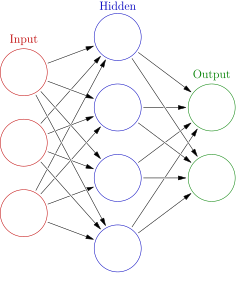
\includegraphics[width=0.9\textwidth]{Colored_neural_network.svg}
	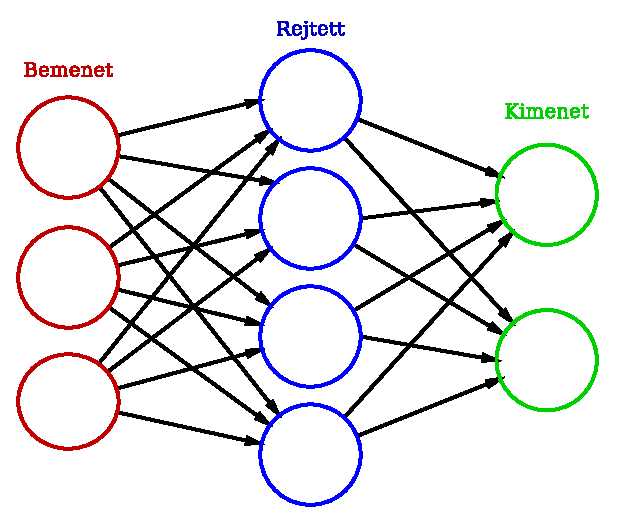
\includegraphics[width=0.3\columnwidth]{fig/neural_network}
	\caption{neurális hálózat réteges szerkezete \protect \footnotemark}
	\label{fig:neuralNet}
\end{figure}
\footnotetext{forrás: https://en.wikipedia.org/wiki/Artificial\_neural\_network}

A \ref{fig:neuralNet} ábrán a csúcsok jelentik a neuronokat és az élek a szinapszisok, melyeken az ingerület vándorol. Egy hálózat 3 nagyobb részre tagolódik:
\begin{enumerate*}[label={\alph*)},font=\bfseries]
	\item bemeneti réteg
	\item rejtett rétegek
	\item kimeneti réteg.
\end{enumerate*}
A bemeneti réteg csúcsai legtöbbször az adatot reprezentáló konstansok jelentik, tehát az egy egyszerű vektor.
Egy neuronban két művelet történik: a bementek összegzése és egy aktiváló függvény kiértékelés. Az összegzést a felsőbb rétegből érkező jelekre elvégezzük:
\begin{displaymath}
	s = \sum_i{w_ix_i} = \vec{w}\cdot\vec{x}
\end{displaymath}
ahol $x_i$ a felső réteg i.-ik neuronjának kimenete, $w_i$ az i.-ik neuron szinapszisához tartozó súly, mellyel a szinapszis "erősségét" határozzuk meg. Az "s" összeghez hozzáadunk még egy $b$ értéket, a neuron aktiválási küszöbértéke lesz.
Az aktivációs függvény adja a neurális hálózat kimenetét, paramétere $s+b$.
A neurális hálózatok fejlesztésekor sokféle függvényt találtak alkalmasnak aktivációs függvény gyanánt. Közös jellemzőjük, hogy inflexiós pontjuk $x=0$ helyen van, illetve 0-ban nem deriválható függvények esetén a töréspont esik ide.

A szemléletesség kedvéért tekintsünk meg az egyrétegű perceptront, vagyis egy egyetlen rétegből álló neurális hálózatot $k$ darab neuronnal. A bemenet legyen az $\vec{x}=(x_1,\dots,x_n)$ vektor (a gyakorlatban bemeneti rétegként szokták hívni). A szinapszisok súlyait a $W=\{w_{ij}:i=1\dots n,j=1\dots k\}$  mátrix ($\vec{w}_i$ az i. bemeneti adatból kiinduló szinapszisokhoz tartozó súlyok vektora lesz), a neuronok küszöbértékeit a $\vec{b}=(b_1,\dots,b_k)$ tartalmazza. Az aktivációs függvény $f$. A hálózat kimenetét, vagyis a  $\vec{y}=(y_1,\dots,y_k)$ elemeit megkapjuk a következőképpen:
\begin{displaymath}
	y_i = f(\vec{w}_i\cdot\vec{x}+b_i)
\end{displaymath}

A fentiekből látszik, hogy a hálózat tervezésénél annak négy tulajdonságát kell meghatároznunk:
\begin{enumerate*}
	\item a rétegek és azok neuronjainak számát
	\item a neuronok aktivációs függvényét (rétegenként egy típusú függvény az összes neuronra)
	\item a szinapszisok súlyát ($W$)
	\item a neuronok aktiválási küszöbét ($\vec{b}$).
\end{enumerate*}
Minden réteghez külön $W$ mátrixot és $\vec{b}$ vektort kell meghatározni. \textbf{Az egyszerűség kedvéért az egy réteghez tartozó $W$-t és $\vec{b}$-t együttesen nevezzük a réteg \emph{súlyainak}}. Ez nagyon sok külön meghatározandó változót jelent, tehát csak az 1. és 2. tulajdonság meghatározása elvárható. Kell egy algoritmus, mellyel az egész hálózathoz tartozó paraméterek sokasága -- vagyis minden réteg súlyának paraméterei -- meghatározható.


\section{Deep Learning}
A Deep Learning-ről szerzett tudásom javát F. Cholett könyvéből\cite{Chollet} szereztem, melynek a témához kapcsolódó részleteit alább bemutatom.

A gépi taunlás egy teljesen más programozási paradigmát jelent, ugyanis a klasszikus programozás során a feldolgozandó adatokhoz a programozó adja az adat feldolgozásának szabályait, amit végig követve a gép kiszámítja a kívánt eredményt. Ezzel szemben a gépi tanulás során a programozó az adathoz  a kívánt eredményt adja meg, amiből a gép felállítja a megoldáshoz vezető szabályokat.%\cite{Chollet}

A Deep Learning más néven a mély tanulás a gépi tanulás egy fajtája. Chollet szerint a név arra utal, hogy a kezdeti adaton több transzformációt végrehajtva egymás után egyre közelebb kerülünk egy olyan reprezentációhoz, ami megfelel a kívánalmainknak. Ezzel kontrasztban beszélhetünk sekély tanulásról, amikor kevés, egy vagy két transzformáció után kapjuk meg az adat megfelelő reprezentációját.%\cite{Chollet}
A neurális hálózatok rétegeltsége adja a \emph{mélységet} a gépi tanulásban. Eredeti elgondolás szerint minden egyes neuron-réteg egyre összetettebb tulajdonságokat ismer fel a bemeneti adatból. Valójában a rétegenkénti transzformációk egyre kisebb összetettségű hipotézis térbe visznek át, a reprezentáció egyre kevesebb -- a felhasználó számára fölösleges -- információt tartalmaz. Minél több réteg van a hálózatban, annál \emph{mélyebb} a modell.

\begin{figure}[h]
	\centering
	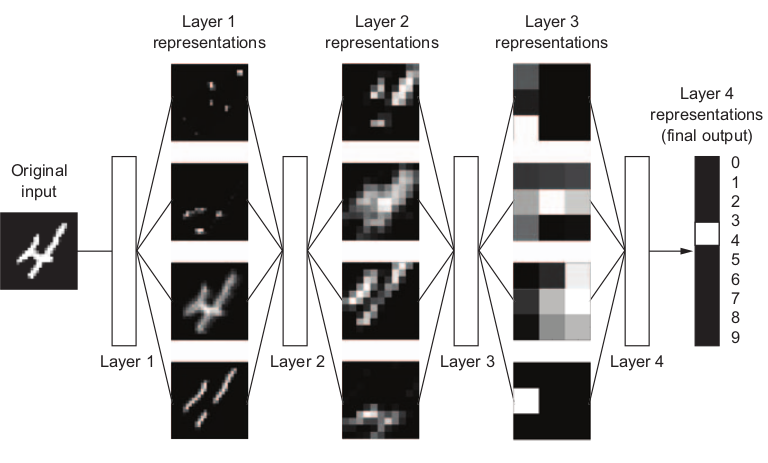
\includegraphics[width=0.8\columnwidth]{fig/digit_classification.png}
	\caption{Írott szám hozzárendelése az ábrázolt számértékhez}
	\label{fig:digit_classification}
	\footnotemark
\end{figure}
\footnotetext{Forrás:\protect\cite{Chollet}}

Itt kapcsolódik össze a neurális hálózat és a mély tanulás. Az \ref{sect:neuralNetworkTheory} alfejezetben kifejtettem, hogy a neurális hálózat szinapszisainak paraméterezéséért felelős $\vec{w}$ súlyok és a neuronok küszöbszintjének állítására szolgáló $\vec{b}$ vektorok összes koordinátájának száma hatalmas lehet, ---alkalmazástól függően több százezer, akár millió, egymástól független változóról beszélünk--- tehát beállításukhoz valamilyen algoritmusra van szükség. Ezért a neurális hálózatok másik komponense, egy tanulási algoritmus, mely beállítja ezen paramétereket. Négy  megközelítés létezik, amikor gépi tanulásról van szó.

\emph{Ellenőrzött tanulás} során a neurális hálózatnak felcímkézett adatokat adunk meg, tehát olyan $y$ értéket  rendelünk az $x$ mintákhoz, amilyet szeretnénk, hogy a hálózat produkáljon. Ezen $z=(x,y)$ összerendezések halmazát \emph{tanítókészletnek} hívjuk. A hálózat leképezi az adatot a meghatározott reprezentációvá. A tanuló algoritmus ebből és a címkéből egy \emph{veszteség függvény} kiszámításával meghatározza, hogy mekkora az eltérés, a valamilyen értelemben vett távolság a kapott és az elvárt eredmény között. Ez alapján frissíti a $\vec{w}$ súlyokat és $\vec{b}$ vektorokat.

\emph{Ellenőrizetlen tanulás}, mely során az adatokat nem címkézzük fel, hanem arra vagyunk kíváncsiak, hogy miféle összefüggések állnak fenn közöttük. Ezt a módszert adatbányászat során alkalmazzák. 

Az \emph{Önellenőrzött tanulás} hasonló az ellenőrzötthöz, azonban az adatok felcímkézését nem emberi erővel végezzük, hanem az adatokból állítjuk elő valamilyen heurisztikát felhasználva. Egyik alkalmazási területe az autóenkóderek tanítása.

A \emph{Megerősítéses tanulás} egy újfajta megközelítése a neurális hálózatok alkalmazásának. Ennél a metodikánál a hálózatot egy ágens alkalmazza, így a hálózat bemenete az ágens által megfigyelt környezet a kimenete pedig valamilyen cselekedet, beavatkozás és tanítás során az ágens igyekszik valamilyen környezetbeli értéket maximalizálni. Gyakori alkalmazás valamilyen játékot játszó ágens, ahol azt tanulja, adott helyzetekre milyen reakcióval tudja maximalizálni játékbeli pontszámát.
Vizsgálódásomat az \emph{ellenőrzött tanulásra} korlátoztam, így a továbbiakban ennek tükrében folytatom dolgozatomat.

\section{Függvények, algoritmusok}\label{sec:fuggvenyek-algoritmusok}
Az alábbiakban szeretném megfogalmazni a neurális hálózatokban alkalmazott tipikus függvényeket és algoritmusokat.
%TODO Kicsit rövid
\subsection{Neuronok aktivációs függvényei}
Mint korábban kifejtettem minden neuron kimenete egy függvény kiértékelése, melynek paramétere a bemenetek súlyozott összege. Ezt a függvényt hívjuk aktivációs függvénynek. 

\paragraph{A szigmoid függvény}
Az utolsó, kimeneti neuronok rétegének aktivációs függvényeként alkalmazzuk, ahol a várt eredmény egyetlen valószínűségi érték. Ez bináris osztályozási problémák esetén alkalmazandó, tehát a program célja, hogy egy bemeneti adatról eldöntse, hogy az egy bizonyos kategóriába esik-e vagy sem, illetve erről mekkora "magabiztossággal" döntött.
\begin{equation}
	\sigma(x)= \frac{1}{1+e^{-x}}
	\label{eq:sigmoid}
\end{equation}\

\paragraph{A softmax függvény}
A kimeneti réteg aktivációs függvénye. $D$ dimenziójú $x$ vektorok koordinátáit normalizálja, másként fogalmazva egy tetszőleges $D$ elemű szám n-est azon $D$ elemű n-esek halmazába képezi, melyek elemeinek összege 1. Így tehát a $x$ koordinátái egy diszkrét valószínűségi eloszlás értékkészlete. 
\begin{equation}
\sigma(x_i)=\frac{e^{x_i}}{\sum_{j=1}^{D}e^{x_i}},\quad i = 1,\dots,D
\label{eq:softmax}
\end{equation}
Éppen ezért többosztályos problémáknál használatos.A hálózat egy mintára adott válasza annak a diszkrét valószínűségi változónak az eloszlása, mely a minta egy adott kategóriába tartozásának a valószínűségét adja meg.

\paragraph{ReLu}
Teljes néven \emph{rectified linear unit} függvény vagy közismerten rámpafüggvény a rejtett neuron rétegek aktivációs értéke szokott lenni. Először 2011-ben mutatták be, hogy hatékonyabban taníthatóak a neurális hálózatok, mintha csak szigmoid függvényt használnánk neuronok aktivációs függvényeként.\cite{wiki:relu}
\begin{equation}
	f(x) = max{0,x}
	\label{eq:relu}
\end{equation}

\begin{figure}[h]
	\centering
	\begin{subfigure}[b]{0.3\textwidth}
		\def\svgwidth{0.5\columnwidth}
		\input{fig/Logistic-curve.pdf_tex}
		\caption{Szigmoid függvény}
		\label{fig:sigmoid}
	\end{subfigure}
	~
	\begin{subfigure}[b]{0.3\textwidth}
		\def\svgwidth{0.5\columnwidth}
		\input{fig/Ramp_function.pdf_tex}
		\caption{ReLu függvény}
	\end{subfigure}
	\caption{Aktivációs függvények }
\end{figure}

\subsection{Veszteség függvények}
A neurális hálózat tanításához szükséges meghatároznunk egy $c(\vec{y},\vec{y'})$ veszteségfüggvényt, mely megadja a hálózat kimenetének eltérését az elvárt eredményhez képest adott súlyok mellett. Ezt az eltérést egy skalárértékként képezi le.
%Formálisan egy $c:W\times B \mapsto \mathbb{R}^+$ függvény, $W,B$, a súlyokat és küszöbértékeket egybefogó vektorok halmaza. Ezen többváltozós függvény képe a \emph{veszteségfelület}.
%TODO c(w,b) vagy c(y,y') helyes megközelítés?

\paragraph[MSE]{Átlagos négyzetes hiba}
Többosztályos problémánál a neurális hálózat egy valószínűségi változó eloszlása az összes osztályon. $\vec{y}$ vektor a hálózat válasza a $\vec{x}$ bemenetre, $\vec{y'}$ pedig a kívánt kimenet vektora --egy egységvektor, melynek 1 értékű koordinátája reprezentálja a megfelelő osztályt. Erre az esetre olyan veszteségfüggvényt alkalmazhatunk mely ekvivalens a $(\vec{x},\vec{y})\in Z$ tanítási készletből számított $MSE$ átlagos négyzetes hibáinak átlagával.
\begin{align*}
	MSE(\vec{y},\vec{y'}) = \frac{1}{n}\sum_{i=1}^{n} (y_i - y'_i)^2\\
	C(w,b) = \frac{1}{m}\sum_{j=1}^{m} MSE(\vec{y}_j,\vec{y'}_j)\\
\end{align*}
A fenti egyenletekben n az kimeneti vektor dimenziója, m a tanító minták száma.
	%
	%\begin{displaymath}
	%	C(w,b)\equiv\frac{1}{2n}\sum_x\|y-y'\|^2\quad\footnote{forrás\cite{Nielsen2015}}
	%\end{displaymath}
%TODO nézd át

\paragraph{Kereszt-entrópia}
Osztályozási feladatoknál olyan módszert használhatunk a veszteség  vagy hiba érték számításához, melynél az $\vec{y}$ és $\vec{y'}$  kereszt entrópiáját határozzuk meg. Ilyen jellegű feladatoknál az említett vektorok valószínűségi eloszlások.
\begin{displaymath}
	H(y,y')= -\sum_{x\in \mathcal{X}}y(x)\log y'(x)
\end{displaymath}

A mély tanuláshoz használt keretrendszereknél gyakran másként implementálják a kereszt-entrópiát kétosztályos és többosztályos esetre. Ezekre az implementációkra \emph{bináris kereszt-entrópia} és \emph{kategorikus kereszt-entrópia} néven hivatkoznak.

\subsection{A hálózat tanító algoritmusai: az optimalizálók}
Korábban említettem, hogy egy neurális hálózat tanításán azt az eljárást értjük, amely során a hálózat paramétereit változtatjuk. Neurális hálózatoknál gradienscsökkentésen alapuló technikákat alkalmazunk. A módszer alapját az az elképzelés adja, hogy a meghatározunk egy $C(\vec{w}_1,b_1,\dots,\vec{w}_L,b_L)$ függvényt, mely a hálózat összes paramétere alapján meghatároz egy $E$ hibaértéket, ami a tanítási folyamat egy ciklusa során kapott veszteségértékek átlaga. Ezen függvény képe egy úgymond \emph{hibafelület}, melynek megkeressük  minimum helyeit tanítás során. Gyakorlatban nem kivitelezhető a globális minimum meghatározása, és lokális minimumok keresését is iteratív módszerekkel célszerű végezni. Többváltozós függvények esetén a gradiens vektor ellentettje ($-\nabla f$) segítségével meghatározható, hogy adott pontban -- azaz megadott függvényparaméterek esetén -- a paramétereket milyen mértékben változtassuk, hogy a függvény kimeneti értékét a legdrasztikusabb mértékben csökkentsük.

Belátható, hogy $C$ ekvivalens a $c$-k átlagával.
\begin{align*}
\frac{1}{n}\sum_{i=1}^{n}c(y_i,y'_i) \equiv C(\vec{w}_1,b_1,\dots,\vec{w}_L,b_L)\\
\end{align*}
A gradienscsökkentés naiv megközelítése pedig a következő:
\begin{align*}
	\vec{W_i}=(\vec{w_i}_1,b_{i1},\dots\vec{w_i}_L,b_{iL})\\
	\vec{W_{i+1}} = \vec{W_i} - \nabla C(\vec{W_i})
\end{align*}
Ahol $\vec{W_i}$ a tanítás i-edik ciklusában az $L$ rétegű hálózat összes paraméterének vektora.

\begin{figure}[h]
	\centering
	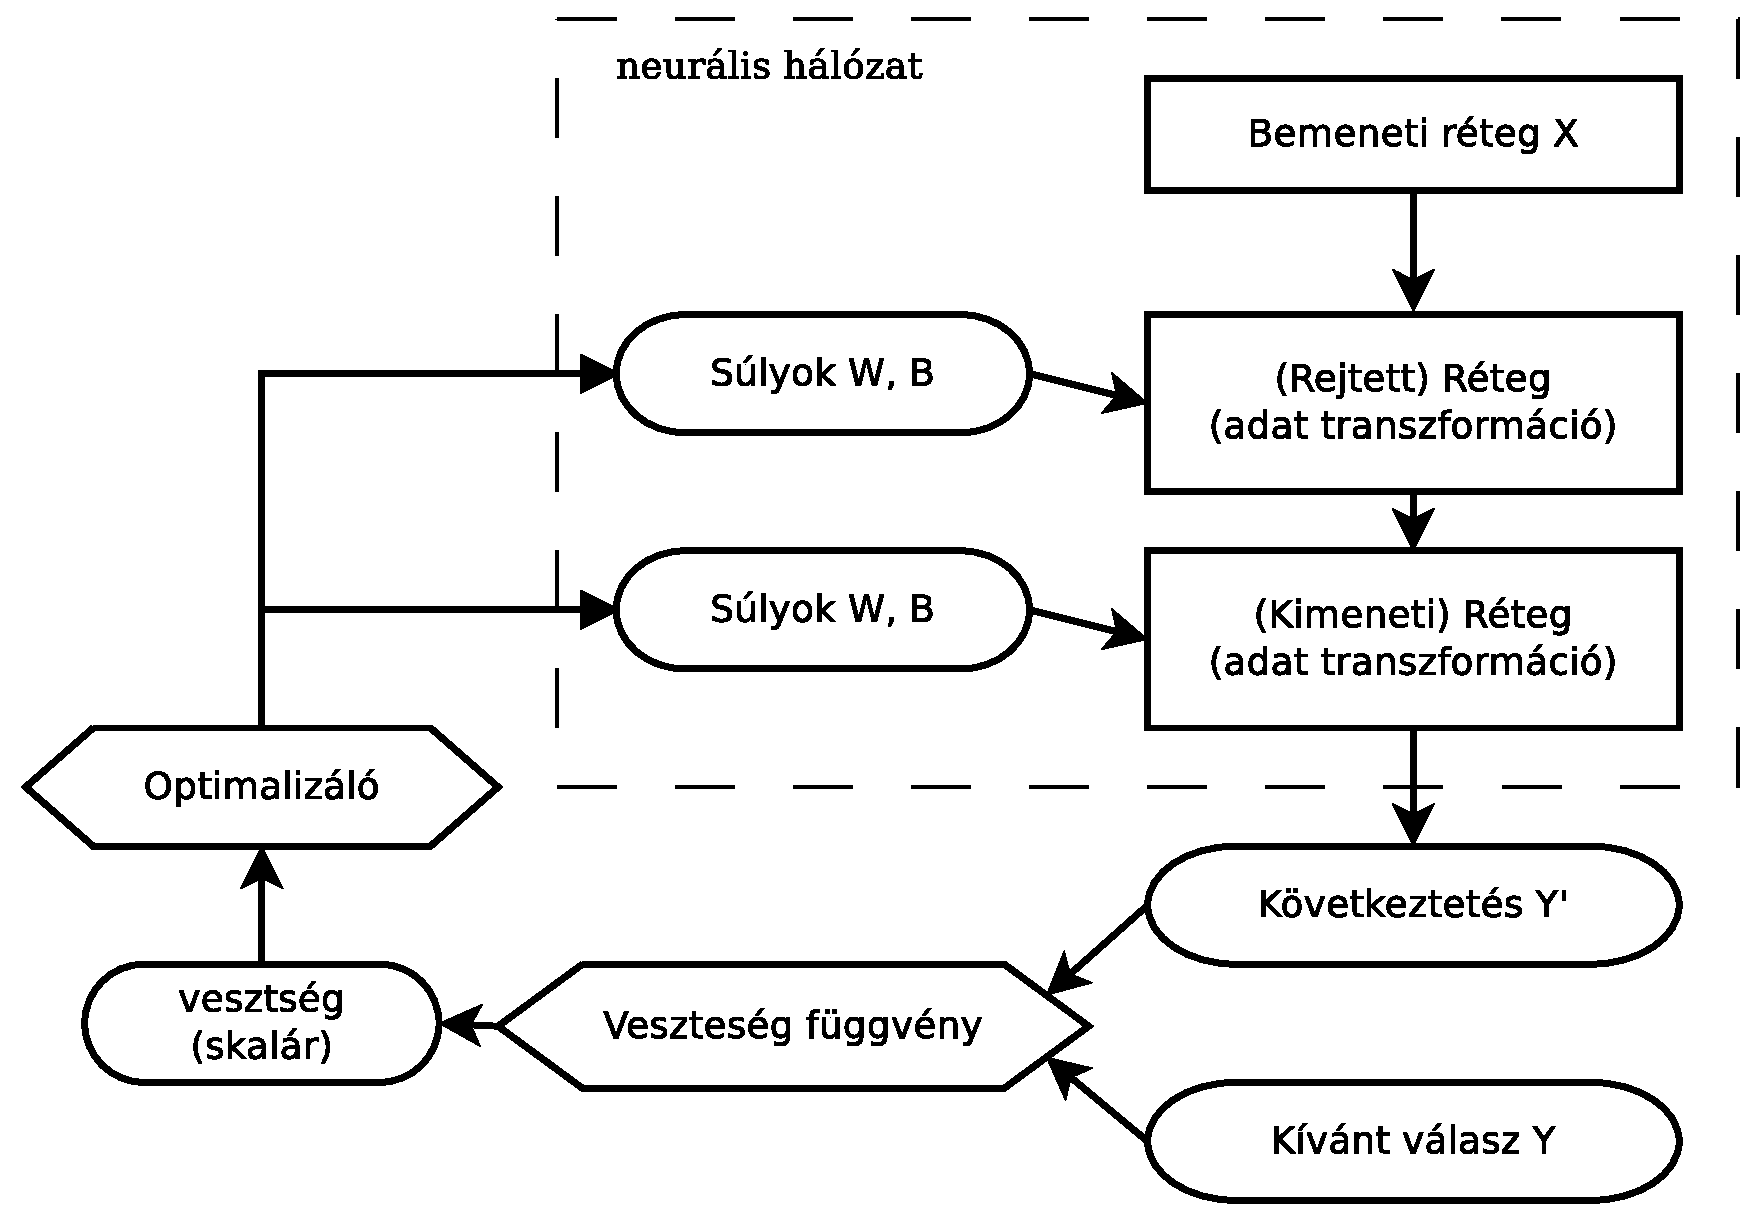
\includegraphics[width=0.7\linewidth]{fig/DNN_dia}
	\caption{A neurális hálózat tanításának folyamata}
	\label{fig:dnn}
\end{figure}

A tanítási folyamat iterációit \emph{eposzoknak} (angolul: epoch) nevezi a szakirodalom. Minden eposzban az optimalizáló hatására a kimeneti hiba csökken, a hálózat \emph{következtetése} egyre közelebb kerül az elvárthoz. 

\paragraph[SGD]{Sztochasztikus gradienscsökkentés}
A naiv megközelítést alapul véve meghatározunk egy $\eta$ tanítás sebességet (angolul: learning rate), mellyel azt befolyásoljuk, hogy egy eposzban a hálózat paramétereit mekkora mértékben változtatjuk. A tanítási sebesség az optimalizálók egy másik paramétere, tehát más eljárás esetén is alkalmazzuk valamilyen formában.
\begin{displaymath}
\vec{W_{i+1}} = \vec{W_i} - \eta\nabla C(\vec{W_i})
\end{displaymath}
Ezen paraméter változtatásánál fontolóra kell vennünk két tényezőt. Nagy tanítási sebesség gyorsabb gradiens csökkenést eredményez, ugyanakkor az elmozdulás a hibafelületen nagy kitérésekkel történik a minimumpont irányába. Túl kicsi tanítási sebességgel -- azon túl, hogy megnövekszik az eposzok szám --  ugyanakkor az optimalizálás "beragadhat" egy kedvezőtlen lokális minimum helyen.

\paragraph[RMSprop]{négzetes közép visszaterjesztése}
%RMSprop -> Root Mean Square propagation
Konstans tanulási rátát nehezen lehet jól megválasztani, ezért olyan eljárásokat dolgoztak ki, ahol ezen érték adaptálódik a tanítási folyamat során, hogy kiküszöbölje az előző bekezdésben említett nagy kitéréssel történő konvergenciát és a "beragadást". Az egyik ilyen módszer az, hogy a tanulási rátát elosztjuk az előző ciklusokban számított gradiensek nagyságának négyzetes közepével.
$$ v(w,y) = \gamma v(w,y-1) +(1-\gamma)(\nabla C(W_i))^2 $$
Ahol $\gamma$ az ún. felejtési tényező amivel szabályozhatjuk, hogy mekkora befolyása legyen az újabb gradienseknek.\\
A hálózat paramétereit a következőképpen frissítjük:
$$ W_{i+1} = W_i - \frac{\eta}{\sqrt{v(w_,y)}} \nabla C(W_i) $$


%TODO Nincs Befejezve
\subsection{A kernel-trükk}

%TODO Nincs Befejezve
%-------------------------------------------------------------------------------
\chapter{Mélytanulásos alkalmazások fejlesztése}
%-------------------------------------------------------------------------------
% TODO: Mélytanulásos keretrendszerek bemutatása általánosságban (mire jók, stb...)
\section{Keras}

\section{TensorFlow}


%-------------------------------------------------------------------------------
\chapter{Specializált hardver megjelenése}%{Célprocesszorok megjelenése}
%-------------------------------------------------------------------------------
\section{hybrid deep learning}
A ha

\section{nGraph}
A most leírtak alapját az nGraph hivatalos dokumentációja adja\cite{web:ngraph_intro}.
Az nGraph az Intel\registeredlogo által fejlesztett programkönyvtár és egy futtatási környezet/fordító készlet 
melyet mélytanulásos projektekhez.
Legszembetűnőbb tulajdonsága, hogy képes többféle hardver architektúrán futtatni és beépíthető számos keretrendszerbe.
Ezek azok a jellemzők, amiket kerestünk témavezetőmmel, hogy mélytanulást tudjunk végeztetni hatékonyan a \emph{HuSSar-on}. 
Ezen túlmenően a jövőbeli fejlesztések az iparban egyre jelentősebben igényelik, hogy a modern MI rendszerek skálázhatóak legyenek, mert egyrészt a neurális hálók egyre komplexebbé válnak, másrészt az általuk feldolgozott adatok mennyisége is rohamosan növekszik.

Jelenleg két bevett gyakorlat van a mélytanulás felgyorsítására:
\begin{enumerate}
	\item \textbf{Dedikált hardver tervezése a mélytanulásos számításokhoz} -- Sok vállalkozás tervez \emph{Alkalmazásspecifikus integrált áramköröket} (ASIC) neurális hálózatok betanítására és futtatására.
	\item \textbf{Szoftver optimalizáció} -- Programkönyvtárakat tartalmazó fejlesztési keretrendszerek fejlesztése, melyek képesek a hálózatokkal kapcsolatos számításokat több szálon, optimalizáltan futtatni. Az nGraph, mint fordító is egy ilyen megoldás.
\end{enumerate}

\subsection{Motiváció}
A mai legmodernebb szoftveres megoldás mélytanulásra az, ha integrálunk kernel könyvtárakat\footnote{Programkönyvtár, mely neurális hálókkal kapcsolatos elemi, \emph{mag} függvényeket tartalmazzák} mélytanulásos keretrendszerekbe.
Ilyen integráció lehet például ha a Tensorflow keretrendszer alatt az Nvidia CuDNN könyvtárát használjuk.
A {kernel könyvtárak} egy adott célarchitektúrára optimalizált kernelekből és egyéb műveleti szintű optimalizálásokból állnak, ezekkel érve el teljesítménynövekedést.
Azonban a kernel könyvtáraknak három fő problémája van:
\begin{enumerate}
	\item Nem biztosítanak gráf szintű optimalizálást
	\item A keretrendszerek integrációja a {kernel könyvtárakkal} nem skálázható
	\item A szükséges lefordított kernel könyvtárak száma növekszik, ahogy új processzorok jelennek meg
\end{enumerate}
Az nGraph fordító megoldás az első két problémára, és a \emph{PlaidML}-el ötvözve kiküszöbölhető a harmadik probléma.
\subsection{Gráf szintű optimalizálás}
Az nGraph dokumentációjában áll egy példa arra vonatkozóan, hogyan lehet, hogy egy mélytanulásos keretrendszer integrálva egy {kernel könyvtárral} a számításokat optimálisan végzi, mégis a számítási gráf a csúcsait alkotó műveletek szempontjából mégsem optimális.
\begin{figure}[!ht]
	\centering
	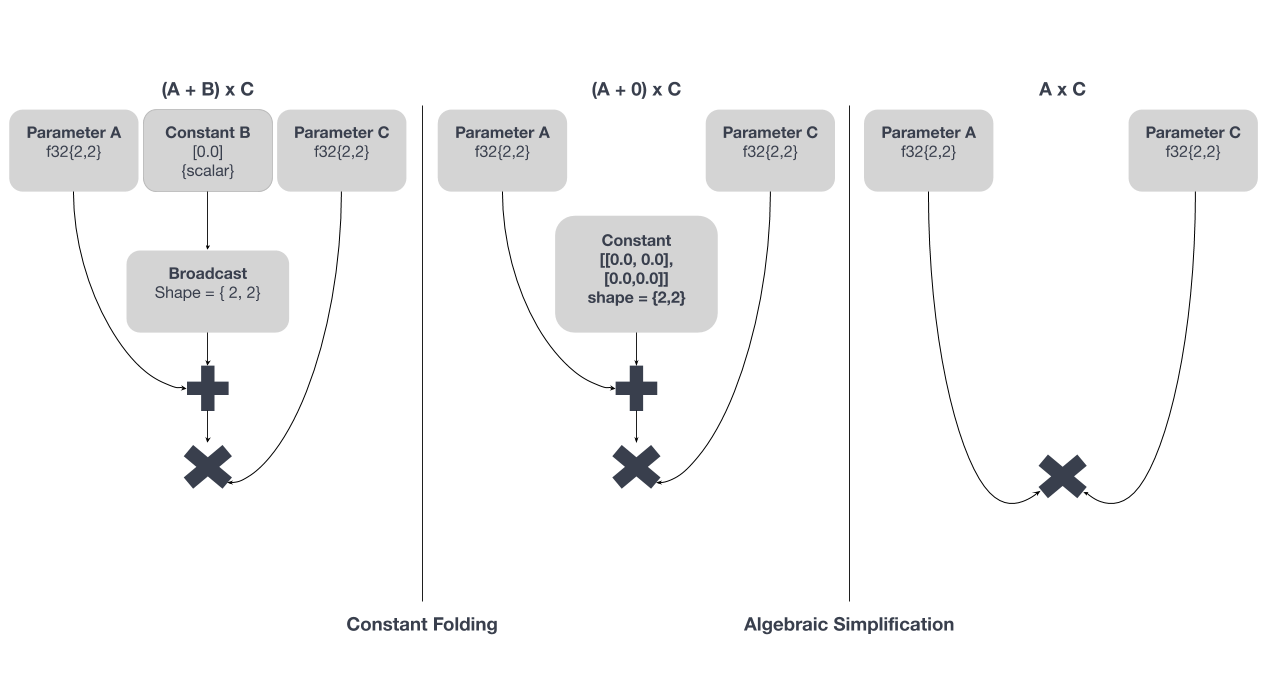
\includegraphics[width=0.9\textwidth]{kernel-problem-1.png}
	\caption{két optimalizálás módszer: konstans összehajtás és algebrai egyszerűsítés a gráfon. \protect \footnotemark}
	\label{fig:grafoptimalizalas}
\end{figure}
\footnotetext{forrás: \cite{web:ngraph_intro}}
A fenti ábra bemutatja, hogyan egyszerűsíthetünk az $A$,$B$ és $C$ tenzorokat feldolgozó, $ (A+B)*C $ tenzorműveletet végrehajtó számítási gráfon.
Fordítási időben megállapítható, hogy $B$ egy skalár konstans, így a \emph{konstans összehajtásnak} nevezett optimalizálás elvégezhető, és a 2 dimenziós vektorrá való kiterjesztés művelete elhagyható (helyette inkább közvetlenül létrehozunk egy $2\times2$ tenzort).
Ebben a példában $B=0$ skalár volt, így a belőle létrejött tenzor egy nullmátrix, így az semleges a kifejezés kiértékelésének szempontjából.
\emph{Algebrai egyszerűsítést} végezve az $ (A+0)*C $ leegyszerűsíthető az $A*C$ kifejezésre, így összesen két csúccsal csökkentettük a gráfunkat.
Ez az optimalizáció tehát a számítási gráf szintjén lett elvégezve.
Így belátható, hogy a mélytanulásos keretrendszerbe integrált kernel programkönyvtárak nem optimális futást végeznek, hiába a műveletek szintjén elért optimalizálás. 
\subsection{Skálázható keretrendszer integráció}
Ahogy gyarapodik a mélytanuláshoz használható gyorsítókártya architektúrák és keretrendszerek száma, a meglévő mélytanulást alkalmazó fejlesztési platformok bővítése egyre több munkát igényel és egyre nő a hibák megjelenésének a valószínűsége. Az integráció kapható készen, szakértő fejlesztőcsapatoknak kell implementálnia.
Minden új keretrendszert manuálisan kell integrálni a meglévő hardverek kernel könyvtárával és minden újonnan megjelenő hardvercsalád meghajtó programkönyvtárát be kell integrálni egyesével a meglévő keretrendszerekbe.
Ez a munka önmagában is hatalmasra tud nőni, de egy sok eszközből álló összeállítás nagyon törékeny és költséges a fenntartása.
Az nGraph úgy oldja meg ezt a problémát, hogy ún. \emph{hidakat} alkalmaz, amikkel integrálható valamelyik mélytanulásos keretrendszerbe.
A híd megkapja a keretrendszerben megalkotott számítási gráfot vagy ahhoz hasonló struktúrát és átalakítja egy ún. \emph{közbenső reprezentációvá}\footnote{IR: Intermediate Representation}. Ezzel kaptunk egy egységes, platformfüggetlen számítási gráfot, így nem kell egy új programkönyvtárat beintegrálni minden egyes meglévő keretrendszer alá, elegendő csak az, hogy az nGraph-ban, mint programkönyvtárban implementált \emph{primitív műveleteket} támogassa az új programkönyvtár.
\subsection{Növekvő kernel szám}
Egy kernel könyvtár integrálása egyszerre több mélytanulásos keretrendszerrel nehéz feladat és egyre komplexebbé válik, ahogy növekszik az optimális teljesítményhez szükséges kernelek száma.
Régen a mélytanulásos kutatások egy kis számú \emph{primitív} számítást használtak, mint a konvolúció, általános mátrixszorzás, stb. Az MI kutatás előrehaladtával és az ipari mélytanulásos alkalmazások továbbfejlesztésével, a szükséges kernelek száma (k) exponenciálisan nő.
Ez a szám a processzor architektúrák számán (h), adattípusokon (t), műveleteken (p) és az egyes paraméterek számosságán (p) alapul ($ k = h \times t \times m \times p $).
\begin{table}[!ht]
	\centering
	\begin{tabular}{|c|c|c|c|}
		
		Hardver & Művelet & Adattípus & Paraméterek \\ 
		\hline
		CPU & konvolúció & 16 bites lebegőpontos & NCHW vagy NHWC \\ 
		
		GPU & MatMul & 32 bites lebegőpontos & 2D, 3D és 4D tenzorok \\ 
		
		FPGA & Normalizálás & 8 bites egész &  \dots \\ 
		
		\dots & \dots & \dots & \\
	\end{tabular} 
	\caption{Néhány példa, tényezőnként hányféle esetre kell külön fordítani  kernelt könyvtárt }
	\label{table:kernels}
\end{table}

Ezen probléma megoldásához jön képbe a PlaidML. Ez egy \emph{tenzor fordító}\footnotemark, mely azt célozza, hogy képes legyen neurális hálózatokat tanítani és futtatni bármilyen típusú hardveren. Más szavakkal segíti a magas szintű keretrendszerek (Keras, ONNX, nGraph) integrálni olyan ezsközökkel, melyekhez nincs meg a szükséges támogatás vagy a meglévő szoftverkészlet hozzájuk szigorúan linceszelt.\cite{github:PlaidML}\cite{web:PlaidML}
\footnotetext{Olyan fordító, melynek nyelve arra lett fejlesztve, hogy főleg tenzorműveleteket igénylő számításokat tudjunk hatékonyan programozni}

Az nGraph tehát integrálható a PlaidML-el. Elsősorban az nGraph a platform független IR-rel igyekszik orvolsoni a skálázható backend-el kapcsolatos kihívást. A PlaidML ezt megtámogatja azzal, hogy képes az IR-ből származó gráfokból LLVM, OpenCL, OpenGL, CUDA és Metal kódot generálni melyek a megfelelő hardveren futtathatóak. Így egy magas szintű keretrendszerben írt neurális háló lefordul Intel és AMD processzrokon valamint grafikus processzorokon, az nVidia processzorain, továbbá az Apple cég által feljelsztett eszközökön.

Az nGraph gráf szintű optimalizációját ráadásul kiegészíti automatikusan a PlaidML alacsonyabb szinten, ezzel teljesítmény növekedést érve el.

Összegzésül tehát az nGraph feldarabolja a neurális hálózathoz tartozó számítási gráfot processzor architektúrának megfelelően, majd ezen gráfokat a PlaidML lefordítja a megfelelő kódokra, melyeket aztán a célprocesszorokra lefordítunk és futtatunk.

\section{Myriad X és az Intel Neural Computer Stick 2}

\section{Google ???}


\section{Új gyorsítók: Intel Nervana Neural Network Processor}

%-------------------------------------------------------------------------------
\chapter*{Összefoglalás}\addcontentsline{toc}{chapter}{Összefoglalás}
%-------------------------------------------------------------------------------
%\lipsum[1]
A gépi tanulás olyan területeken jelent meg melyek új kihívásokat szültek. A hardvergyártók kifejezetten deep learningre optimalizált megoldásokat kínálnak és a jövőbeli fejlesztések is ebbe az irányba mutatnak. Ezen dolgozatomban bemutatott, mély tanulásban használatos technológiákon látható, hogy egyre változatosabb deep learning rendszereket alapját tudják nyújtani. Olyan keretrendszerek születtek független fejlesztőcsapatok és a hardvergyártók jóvoltából, melyekkel gyorsan és hatékonyan végezhető mély tanuló alkalmazások fejlesztése. Ennek jóvoltából a mindennapi életben is megjelenik ez a technológia, és azon is túl a kutatásokban megjelenő nehezen megoldható számítási problémák váltak kivitelezhetővé. Ezen technológiákat felölelő szakterületek a munkaerőpiacon is igen keresetté válhatnak.

A hardveripar most is sok erőforrást fektet a gyakorlatban használt mesterséges neurális hálózatok hatalmas számítási igényének kielégítésére. Újabb és hatékonyabb eszközöket kínálnak erre a feladatra. Némelyikük a korábban bevált GPGPU architektúrák továbbfejlesztése, míg mások speciális, csakis kifejezetten deep learning architektúrák. Ezek az eszközök a több magos masszívan párhuzamos számításokra alapoznak, melyek jól alkalmazhatóak a neurális hálózatokon.

Ezzel párhuzamosan hibrid számítási rendszereket támogató keretrendszerek is készülnek, szintén a párhuzamos számítás modellre, azontúl az egyes architektúrák eltérő működésére alapozva. Ennek köszönhetően a deep learning alkalmazások változatos hardver architektúrákon futtathatóak, melyek a nyers erőn túl a számítások hatékony végrehajtásával érnek el teljesítménynövekedést. Az ilyen technológiák továbbá lehetőséget biztosítanak, hogy a felhasználók meglévő hardvereiket építsék be deep learning rendszerekbe. Ez a fejlesztési költségek szempontjából nagyon előnyös, ezért a jövőben várhatóan egyre több szerveren találkozhatunk tanuló vagy tanítható alkalmazásokkal.

A nagygépes világgal párhuzamosan megjelentek külön mély tanulásra specializált integrált áramkörök a hordozható és személyi eszközökön is. A Deep Learning így egy ,,kézzel fogható'' technológiává válik. Ez az irány elősegíti a valós idejű mély tanuló alkalmazások fejlesztését, mint például az önvezető járművek, intelligens gyártósorok, személyi applikációk vagy egyes orvosi alkalmazások. Úgy látszik a jövőben erre a szolgáltatók is számítanak: ezen speciális hardverek némelyike építőkövei lehetnek az ún. \emph{Edge Computing} modellnek: míg kezdetben a felhőszolgáltatásokat nyújtó vállalatok neurális hálózatai teljes egészében szervereiken futottak, mára kezd kibontakozni az az elképzelés, hogy ezeket a számításokat a felhasználóhoz egészen közel lehet vinni, így közel valós idejűek lehetnek a felhő alapú deep learning szolgáltatások is a jövőben.

A szakdolgozatom írása során rengeteg új ismeretre tettem szert. Igyekeztem a legmodernebb hardvereket és legújabb szoftverfejlesztéseket felkutatni. Így szembesültem azzal is, hogy ennek a szakterületnek csak felszínét vizsgáltam még. Ahhoz, hogy tényleg jó rálátásom legyen a jövőbeli fejlesztésekre, a gépi tanulással kapcsolatos ismereteimet mesterképzésben szeretném elmélyíteni.
%A szakdolgozatom készítésének elején végzett kísérleteim az nGraph-fal kudarcba fulladtak, annak félkész mivolta miatt. Azonban reménykedve fejlesztés eredményességében a jövőben újra megkísérlem ...
\clearpage

% irodalomjegyzék
%---Hagyományos---
%----------------------------------------------------------------------------
%Irodalomjegyzék
%----------------------------------------------------------------------------
\begin{thebibliography}{9}
%Könyvek,cikkek,tanulmányok
\bibitem{Chollet}
	François Chollet,
	\textbf{Deep Learning with Python},
	Manning Publications,
	2018.

\bibitem{neural2006}
	Altrichter Márta \& Horváth Gábor \& Pataki Béla \& Strausz György \& Takács Gábor \& Valyon József,
	\textbf{Neurális hálózatok},
	Panem,
	2006,
	[Szakkönyv],

\bibitem{mccullogh1943}
McCulloch, W.S. \& Pitts, W.,
\textbf{A Logical Calculus of Ideas Immanent in Nervous Activity},
Bulletin of Mathematical Biophysics,
1943,
doi:10.1007/BF02478259.

%adatforrások

%jogszabályok

%Kézikönyvek

\bibitem{web:PlaidML}
\textbf{PlaidML -- Home},
2019. október 20.,
Vertex.AI.,
\newline\url{https://vertexai-plaidml.readthedocs-hosted.com/en/stable/}

\bibitem{web:ngraph_intro}
\textbf{Introduction --- Documentation for the {nGraph} Library and Compiler stack},
2019,
\newline\url{https://ngraph.nervanasys.com/docs/latest/introduction.html},
[meglátogatva 2019. október 08.]

%Internetes adatgyűjtés

\bibitem{wiki:plaidml}
	\textbf{PlaidML --- {Wikipedia}{,} The Free Encyclopedia},
	2019,
	\newline\url{https://en.wikipedia.org/w/index.php?title=PlaidML&oldid=898300482},
	[meglátogatva 2019. október 5.]


\bibitem{ wiki:constfold}
	\textbf{Constant folding --- {Wikipedia}{,} The Free Encyclopedia},
	2019,
	\newline\url{https://en.wikipedia.org/w/index.php?title=Constant_folding&oldid=914455114},
	[meglátogatva 2019. október 09.]


\bibitem{github:nGraph}
	\textbf{NervanaSystems/ngraph: nGraph - open source C++ library, compiler and runtime for Deep Learning},
	GitHub repository,
	2019,
	\newline\url{https://github.com/NervanaSystems/ngraph},


\bibitem{github:PlaidML}
	\textbf{plaidml/plaidml: PlaidML is a framework for making deep learning work everywhere},
	GitHub repository,
	2019. október 20.,
	\newline\url{https://github.com/plaidml/plaidml},



\bibitem{web:GoogleEdge}
	\textbf{Edge TPU: Hands-On with Google’s Coral USB Accelerator},
	2019. október 23.,
	\newline\url{https://heartbeat.fritz.ai/edge-tpu-google-coral-usb-accelerator-cf0d79c7ec56},

\bibitem{web:Keras}
	\textbf{Keras Dokumentáció}
	2019. október 23.
	\newline\url{https://keras.io/}

\end{thebibliography}
%---Biblatex---
%\bibliographystyle{tex/bibstyle}
%\bibliographystyle{plain}
%\bibliography{bib/bibliography}
%---Biblatex biblatex usepackage-al---
%\printbibliography[heading=bibintoc, title={Irodalomjegyzék}]

% függelék
%-------------------------------------------------------------------------------
\appendix
%-------------------------------------------------------------------------------
\chapter*{Függelék}\addcontentsline{toc}{chapter}{Függelék}
\setcounter{chapter}{6}  % a fofejezet-szamlalo az angol ABC 6. betuje (F) lesz
\setcounter{equation}{0} % a fofejezet-szamlalo az angol ABC 6. betuje (F) lesz
\section{Példa}

%%----------------------------------------------------------------------------
\chapter*{Köszönetnyilvánítás}\addcontentsline{toc}{chapter}{Köszönetnyilvánítás}
%----------------------------------------------------------------------------
Ezúton köszönöm témavezetőmnek biztatását amit a neurális hálózatokkal való ismerkedésem során nyújtott továbbá, hogy mindig számíthattam a segítéségére. A mély tanulás iránti lelkesedésével engem is átitatott, mely átsegített a nehézségeken. Nélküle talán sose ismerkedtem volna meg közelebbről ezzel a területtel. Szeretném továbbá megköszönni szüleimnek azt, hogy mellettem álltak, mikor szakterületet váltottam és támogatták egyetemi tanulmányaimat.

\end{document}